\chapter{Síndrome Metabólico}\label{insulina}

La glucosa es la principal fuente de energía para todos los tejidos del cuerpo humano. Es crucial que los niveles de azúcar en la sangre se mantengan dentro de un rango óptimo de 60 a 120 mg/dl para garantizar un suministro adecuado de energía al sistema nervioso y a todo el organismo \cite{ImgHomeos}.

Para regular estos niveles, el cuerpo cuenta con dos hormonas clave: la insulina y el glucagón. La insulina, producida por el páncreas, juega un papel fundamental en la absorción y utilización de la glucosa por parte de las células del cuerpo. Esta hormona controla la velocidad a la que la glucosa se consume en los músculos, el tejido graso y el hígado, permitiendo que las células obtengan la energía necesaria para su funcionamiento adecuado.

Por otro lado, el glucagón, también producido por el páncreas, actúa en sentido contrario a la insulina. Cuando los niveles de glucosa en la sangre son bajos, el glucagón se libera para estimular la liberación de glucosa almacenada en el hígado, asegurando así un suministro constante de energía cuando es necesario.

Es importante destacar que cada célula del cuerpo utiliza la glucosa de manera diferente, y este uso está determinado por el sistema enzimático específico de cada tipo celular. Esta diversidad en la utilización de la glucosa refleja la complejidad del metabolismo humano y la importancia de mantener un equilibrio adecuado en los niveles de azúcar en la sangre para garantizar un funcionamiento óptimo del organismo.\cite{capitulo4Metabolic}
%%%%%%%%%%%%%%%%%%%%%%%%%%%%%%%%%%%%%%%%%%%%%%%%%%%%%%%
%%%%%%%%%%%%%%%%%%%%%%%%%%%%%%%%%%%%%%%%%%%%%%%%%%%%%%%

\section{Homeostasis de la Glucosa}

La homeostasis de la glucosa, esencial para la vida de los mamíferos, es un proceso complejo que garantiza un equilibrio adecuado de azúcar en la sangre en todo momento. Después de ingerir alimentos, durante el proceso digestivo, la glucosa es absorbida y liberada en el plasma sanguíneo. Este aumento en los niveles de glucosa estimula a las células beta del páncreas a secretar una hormona vital llamada insulina \cite{capitulo4Metabolic}.

La insulina desempeña un papel crucial en la regulación de los niveles de glucosa en la sangre. Actúa disminuyendo los niveles de glucosa en los tejidos periféricos, promoviendo la síntesis de glucógeno en el hígado y en los músculos, y reduciendo la lipogénesis hepática. De esta manera, la insulina ayuda a mantener los niveles de glucosa dentro de un rango óptimo para el funcionamiento del organismo.

Durante el estado de ayuno, cuando no se ingieren alimentos, los niveles de glucosa en el plasma se mantienen entre $4$ y $5$ mM gracias a la acción del hígado, que almacena glucosa en forma de glucógeno. En este estado, los niveles de insulina son bajos y el hígado se convierte en la principal fuente de glucosa plasmática. En este contexto, las células alfa del páncreas producen la hormona glucagón, cuya función es elevar los niveles de glucosa en la sangre mediante la degradación de glucógeno \cite{unamHomeostasis}.

El hígado y las células beta del páncreas son los principales reguladores de las concentraciones de insulina y glucosa en el plasma, en la Figura \ref{fig:homeostasis} \footnote{Imagen tomada de \cite{ImgHomeos}} se ilustra el proceso anteriormente mencionad. Sin embargo, el grado de hiperglucemia puede variar dependiendo de la capacidad de las células beta para secretar insulina y del grado de resistencia a la insulina en el organismo.

\begin{figure}[H]
    \centering
    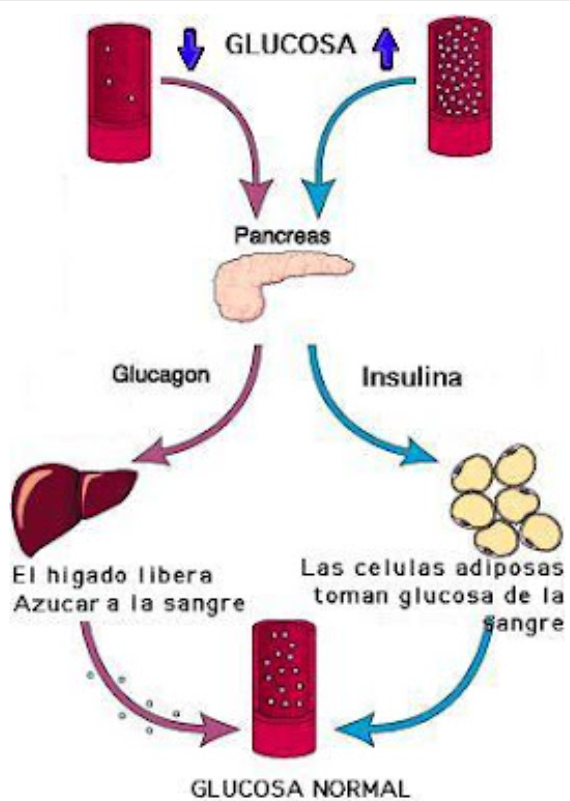
\includegraphics[width = 0.4\textwidth]{homeostasis.png}
    \caption{Esquema General de la Homeostasis de la Glucosa.}
    \label{fig:homeostasis}
\end{figure}

Cuando la homeostasis de la glucosa se ve alterada, se puede desarrollar el síndrome metabólico (SM), un conjunto de condiciones médicas que aumentan el riesgo de desarrollar enfermedades cardiovasculares y diabetes tipo 2. En muchos casos, el SM se presenta cuando las células beta del páncreas se agotan debido a una exposición prolongada a niveles elevados de glucosa en sangre, lo que puede conducir al desarrollo de la diabetes tipo 2. A pesar de los avances en la investigación, este proceso aún no se comprende completamente \cite{capitulo4Metabolic}.

La baja tolerancia a la glucosa en personas sin diabetes se asocia con una respuesta reducida de las células beta a la glucosa, mientras que en personas obesas, esta baja tolerancia se relaciona con una disminución en la sensibilidad a la insulina \cite{computational}. Estas alteraciones en la respuesta metabólica son componentes clave en el desarrollo del síndrome metabólico y la diabetes tipo 2.

Para comprender mejor estos procesos y prevenir las complicaciones asociadas, se han utilizado varios modelos matemáticos para calcular parámetros fisiológicos relacionados con la homeostasis de la glucosa. Estos modelos utilizan datos experimentales para proporcionar una representación matemática precisa de cómo el cuerpo regula los niveles de glucosa en la sangre. Sin embargo, el creciente impacto de la diabetes tipo 2 en la sociedad actual plantea desafíos adicionales, ya que esta enfermedad representa una perturbación significativa en el sistema homeostático de la glucosa \cite{ModelacionMatematica2020}.

%%%%%%%%%%%%%%%%%%%%%%%%%%%%%%%%%%%%%%%%%%%%%%%%%%%%%%%
%%%%%%%%%%%%%%%%%%%%%%%%%%%%%%%%%%%%%%%%%%%%%%%%%%%%%%%%

\section{Resistencia a la Insulina}

La sensibilidad a la insulina y la resistencia a la misma son conceptos fundamentales en el estudio de la fisiopatología de la Diabetes Mellitus (DM). La sensibilidad a la insulina se refiere a la capacidad de los tejidos, especialmente los músculos y los órganos, para responder a la acción de la insulina a través de los receptores de insulina. Por otro lado, la resistencia a la insulina se caracteriza por una disminución en la respuesta de los tejidos a la acción de la insulina, lo que requiere una mayor cantidad de insulina para suprimir la producción de glucosa hepática \cite{MedicionEstimacion}.

En individuos con resistencia a la insulina, se observa una discrepancia entre la concentración de insulina en el plasma y su efectividad para controlar los niveles de glucosa en sangre. En la Diabetes Mellitus, esta resistencia a menudo se presenta junto con altos niveles de glucosa en sangre, lo que puede complicar aún más la regulación de los niveles de azúcar en la sangre.

La causa exacta de la resistencia a la insulina en la DM sigue siendo objeto de debate en la comunidad científica. Se ha sugerido que factores como la obesidad, la inflamación crónica y los factores genéticos pueden contribuir a esta condición. Además, se ha planteado la posibilidad de que la presencia de altos niveles de glucosa en sangre o anticuerpos contra la insulina pueda desempeñar un papel en el desarrollo de la resistencia a la insulina \cite{MedicionEstimacion}.

La Figura \ref{fig:Resistencia}, tomada de \cite{ImgResis}, ilustra este concepto de resistencia a la insulina, mostrando la discrepancia entre los niveles de insulina en el plasma y la respuesta de los tejidos a esta hormona. Esta representación visual ayuda a comprender la complejidad de la relación entre la insulina y la glucosa en el contexto de la Diabetes Mellitus.

\begin{figure}[H]
    \centering
    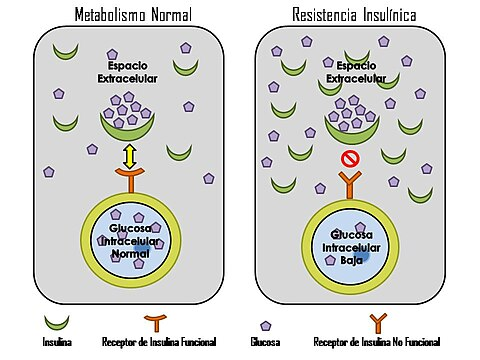
\includegraphics[width = 0.7 \textwidth]{ResisteciaIns.jpg}
    \caption{Resistencia a la Insulina}
    \label{fig:Resistencia}
\end{figure}

Para evaluar la efectividad de la insulina en el organismo, se han desarrollado dos métodos principales: los métodos deducidos y los métodos regresivos. En los métodos deducidos, se utilizan fórmulas derivadas de la lógica y el razonamiento para estimar la sensibilidad a la insulina. Por otro lado, los métodos regresivos proporcionan una fórmula mediante el análisis regresivo de datos experimentales \cite{MedicionEstimacion}.

Una de las pruebas más utilizadas para medir la sensibilidad a la insulina es la prueba de tolerancia a la insulina, también conocida como clamp de insulina. En esta prueba, se administra una cantidad controlada de insulina (0.1 U por kilogramo de peso corporal) y se mide el descenso de la glucosa en el plasma. Sin embargo, este procedimiento puede inducir un estado de hipoglucemia, por lo que se aplica simultáneamente una infusión de glucosa para mantener los niveles de glucosa en sangre en un rango constante. Durante la prueba, se registran los requerimientos de glucosa y la cantidad de insulina necesaria para mantener la homeostasis glucémica. Aunque esta prueba se considera el estándar para medir la sensibilidad a la insulina, su implementación es compleja y se utiliza principalmente en entornos de investigación, no en la práctica clínica de rutina \cite{MedicionEstimacion}.

Dada la complejidad de la prueba de tolerancia a la insulina, se han propuesto otros índices y métodos para evaluar la sensibilidad a la insulina de manera más accesible en entornos clínicos. Estos índices pueden ser útiles para estimar la capacidad del organismo para secretar insulina y para identificar una posible disfunción en el metabolismo de la glucosa.
%%%%%%%%%%%%%%%%%%%%%%%%%%%%%%%%%%%%%%%%%%%%%%%%%%%%%%%

\subsection{Índices de Medición}

Para medir la resistencia a la insulina, se han propuesto varios índices que van desde métodos simples hasta aquellos que toman en cuenta medidas de glucosa e insulina durante pruebas de tolerancia a la glucosa. Algunos de los índices más comúnmente utilizados son el índice HOMA (Homeostasis Model Assessment) o QUICK (Quantitative Insulin Sensitivity Check Index), que se calculan a partir de medidas de glucosa e insulina en sangre en ayunas. Otros índices, como el índice de Matsuda, consideran todas estas concentraciones durante la prueba de tolerancia a la glucosa (OGTT, por sus siglas en inglés) \cite{MedicionEstimacion}.



%%%%%%%%%%%%%%%%%%%%%%%%%%%%%%%%%%%%%%%%%%%%%%%%%%%%%%%

\subsection{Índice HOMA}

El modelo de homeostasis para evaluar la resistencia a la insulina, conocido por sus siglas en inglés como HOMA-IR, es un índice ampliamente utilizado en la investigación para medir la resistencia a la insulina. Fue propuesto por primera vez en 1985 por Rury Holman y David Matthews. Este modelo se basa en la idea de un ciclo de retroalimentación entre las células beta pancreáticas y el hígado.

En el HOMA-IR, la concentración de glucosa en sangre está regulada por la producción de glucosa hepática, mientras que los niveles de insulina en sangre dependen de la respuesta de las células hepáticas a la insulina. Es importante destacar que este índice solo utiliza mediciones de glucosa e insulina en sangre en ayunas. Por lo tanto, una baja respuesta de las células beta a los estímulos de glucosa puede reflejar una deficiencia en la función de estas células, mientras que la resistencia a la insulina se manifiesta como una disminución en la capacidad de la insulina para suprimir la producción de glucosa por parte del hígado \cite{indicesRes}.

El HOMA-IR es una herramienta conveniente y menos invasiva en comparación con el método de clamp de insulina. Se calcula multiplicando la concentración de insulina plasmática en ayunas (FPI) por la concentración de glucosa plasmática en ayunas (FPG), y luego dividiendo el resultado por la constante 22.5, como se muestra en la ecuación:

\begin{equation}\label{HOMAIR}
    HOMA-IR = \frac{FPI \times FPG}{22.5}
\end{equation}

Este índice proporciona una estimación de la resistencia a la insulina y es útil en la investigación clínica y epidemiológica para evaluar el riesgo de diabetes tipo 2 y otras condiciones relacionadas con la resistencia a la insulina.

Además de la evaluación de la resistencia a la insulina mediante el HOMA-IR, también es posible estimar el funcionamiento de las células beta pancreáticas utilizando la ecuación \eqref{HOMAbeta}, conocida como HOMA para las células beta:

\begin{equation}\label{HOMAbeta}
    \text{HOMA células beta} =  20 \times \frac{FPI}{FPG -3,5}
\end{equation}

Esta ecuación proporciona una estimación del funcionamiento de las células beta pancreáticas en relación con los niveles de insulina y glucosa en sangre.

Para interpretar los resultados del HOMA-IR y el HOMA para las células beta, se han establecido valores de referencia. En general, si el valor del HOMA-IR es menor a 1.96, se considera que la sensibilidad a la insulina es adecuada. Si el valor se encuentra entre 1.96 y 2.9, se sospecha de resistencia a la insulina y se pueden requerir estudios adicionales. Finalmente, si el valor es superior a 3, se considera que hay resistencia a la insulina \cite{limiteHOMA}.

Sin embargo, estudios han sugerido que los valores de referencia del HOMA-IR pueden variar entre diferentes poblaciones. Por ejemplo, según el artículo `\textit{The Definition of Insulin Resistance Using HOMA-IR for Americans of Mexican Descent Using Machine Learning}' \cite{HOMAMex}, los valores de referencia para individuos mexicano-americanos son los siguientes: un HOMA-IR menor a 2.6 se considera una sensibilidad normal a la insulina, valores entre 2.6 y 3.8 se consideran en el límite, con posible resistencia a la insulina, y valores superiores a 3.8 indican resistencia a la insulina.

Estas diferencias resaltan la importancia de considerar las características específicas de la población al interpretar los resultados del HOMA-IR y el HOMA para las células beta, y subrayan la necesidad de más investigación para establecer valores de referencia precisos en diferentes grupos étnicos.

%%%%%%%%%%%%%%%%%%%%%%%%%%%%%%%%%%%%%%%%%%%%%%%%%
%%%%%%%%%%% I N D I C E   H O M A  %%%%%%%%%%%%%%
%%%%%%%%%%%%%%%%%%%%%%%%%%%%%%%%%%%%%%%%%%%%%%%%%

\subsection{Índice de Matsuda}

El índice Matsuda de sensibilidad a la insulina ($ISI_{\text{Matsuda}}$) fue propuesto por Matsuda y DeFronzo como una medida de la sensibilidad a la insulina en el organismo. Este índice se calcula utilizando los niveles de glucosa ($mg/dl$) e insulina ($mIU/l$) en sangre tanto en ayunas como durante una prueba de tolerancia a la glucosa oral. La fórmula para calcular el ISI de Matsuda se muestra en la ecuación \eqref{IndexMatsuda}:

\begin{equation}\label{IndexMatsuda}
    ISI_{\textbf{Matsuda}} = \frac{10\;000}{\sqrt{G_0 \times I_0 \times G_{mean} \times I_{mean}}}
\end{equation}

En esta ecuación, $10;000$ es una constante utilizada para obtener un número entre $0$ y $12$, $G_0$ e $I_0$ representan las concentraciones de glucosa e insulina en sangre en ayunas, respectivamente. $G_{\text{mean}}$ es el promedio de las concentraciones de glucosa durante la OGTT, mientras que $I_{\text{mean}}$ es el promedio de las concentraciones de insulina durante la OGTT.

El índice Matsuda de sensibilidad a la insulina tiene un gran poder predictivo para identificar el inicio de la diabetes tipo 2. Al proporcionar una medida de la sensibilidad a la insulina en respuesta a la glucosa, este índice puede ayudar a los médicos a evaluar el riesgo de diabetes tipo 2 en pacientes y a diseñar estrategias de prevención y tratamiento adecuadas \cite{indicesRes}.

%%%%%%%%%%%%%%%%%%%%%%%%%%%%%%%%%%%%%%%%%%%%%%%%%%%%%%%
\subsection{Otros Índices}

Aunque los índices HOMA-IR y Matsuda son ampliamente utilizados en la investigación para evaluar la sensibilidad a la insulina, existen otros índices que también son objeto de estudio. En el artículo "Novel Insulin Sensitivity Index Derived from Oral Glucose Tolerance Test" \cite{NovelInsulin}, se investigó la correlación entre varios índices comúnmente utilizados y la prueba de clamp de insulina, que es considerada el estándar de oro para medir la sensibilidad a la insulina.

En la Tabla \ref{tab:indices} se muestran algunos de estos índices junto con sus respectivas fórmulas. Estos índices fueron evaluados en términos de su capacidad para predecir la sensibilidad a la insulina medida mediante la prueba de clamp de insulina.

\begin{table}[H]
    \centering
    \begin{tabular}{|c|c|}
        \hline \textbf{ Índice } & \textbf{ Ecuación } \\
        \hline \textbf{ HOMA } & $\frac{22.5 \times 18}{I_0  \times G_0}$ \\
        \hline \textbf{ QUICKI } & $\frac{1}{\log (\text { fasting insulin })+\log \text { (fasting glucose) }}$ \\
        \hline \textbf{ Belfiore } & $\frac{2}{(\text { AUC insulin } \times \text { AUC glucose })+1}$ \\
        \hline \textbf{ Cederholm } & $\frac{75,000+(\text { fasting glucose }-2 \text {-h glucose }) \times 1.15 \times 180 \times 0.19 \times \mathrm{BW}}{120 \times \log (\text { mean insulin }) \times \text { mean glucose }}$\\
        \hline \textbf{ Gutt } & $\frac{75,000+(\text { fasting glucose }-2-\mathrm{h} \text { glucose }) \times 0.19 \times \mathrm{BW}}{120 \times \log ([\text { fasting insulin }+2-\mathrm{h} \text { insulin }] / 2) \times[\text { fasting glucose }+2-\mathrm{h} \text { glucose }] / 2}$ \\
        \hline \textbf{ Matsuda } & $\frac{10,000}{\sqrt{(\text { fasting glucose } \times \text { fasting insulin }) \times(\text { mean glucose } \times \text { mean insulin })}}$ \\
        \hline \textbf{ Stumvoll } & $0.22-0.0032 \times \text { BMI }-0.0000645 \times 2 \text {-h insulin }-0.0037 \times 1.5 \text {-h glucose }$ \\
        \hline
    \end{tabular}
    \caption{Índices de Resistencia a la Insulina proveniente de OGTT, tabla tomada de \cite{NovelInsulin}}
    \label{tab:indices}
\end{table}

El artículo \cite{NovelInsulin}, presenta una tabla que muestra los niveles de correlación entre los diferentes índices y la prueba de clamp de insulina. Entre aquellos con mejor desempeño se encuentra el índice Matsuda. Estos resultados ofrecen información importante sobre la utilidad y la precisión de estos índices en comparación con la prueba de clamp de insulina, lo que puede ayudar a los investigadores y clínicos a seleccionar el índice más apropiado para sus estudios o práctica clínica.

Estos índices ofrecen una variedad de enfoques para evaluar la sensibilidad a la insulina y pueden ser útiles en diferentes contextos clínicos y de investigación. Sin embargo, es importante tener en cuenta que cada índice puede tener limitaciones y es crucial validar su utilidad en diferentes poblaciones y condiciones clínicas antes de su aplicación generalizada.


%%%%%%%%%%%%%%%%%%%%%%%%%%%%%%%%%%%%%%%%%%%%%%%%%%%%%%%
%%%%%%%%%%%%%%%%%%%%%%%%%%%%%%%%%%%%%%%%%%%%%%%%%%%%%%%
%%%%%%%%%%%%%%%%%%%%%%%%%%%%%%%%%%%%%%%%%%%%%%%%%%%%%%%

\section{Diabetes}

La Diabetes Mellitus es una enfermedad metabólica crónica que se caracteriza por la presencia de niveles inadecuados de glucosa en sangre. Se han identificado varias subclasificaciones de la enfermedad, que incluyen:

\begin{itemize}
    \item \textbf{Diabetes tipo 1}: Esta forma de diabetes se caracteriza principalmente por la auto destrucción de las células beta del páncreas, típicamente como resultado de un proceso autoinmune. Esto conduce a la destrucción total de las células beta y, por lo tanto, a una deficiencia absoluta de insulina. La diabetes tipo 1 generalmente se presenta durante la niñez o la adolescencia \cite{diabetes}.


    \item \textbf{Diabetes tipo 2}: La diabetes tipo 2 está asociada principalmente con la resistencia a la insulina, una deficiencia relativa de insulina y la presencia de hiperglucemia. Si bien algunos casos de diabetes tipo 2 pueden tener un componente autoinmune, en la mayoría de los casos la enfermedad se desarrolla como resultado de factores como la obesidad y el envejecimiento. Estos factores contribuyen al desgaste en el funcionamiento de las células beta pancreáticas para producir suficiente insulina. La diabetes tipo 2 afecta principalmente a adultos de mediana edad o mayores \cite{computational}.
\end{itemize}

Además de estos dos subtipos principales, existen otras formas de diabetes mellitus, como la diabetes juvenil de inicio en la madurez (MODY), la diabetes gestacional, la diabetes neonatal y la diabetes inducida por esteroides. Sin embargo, este trabajo se enfocará principalmente en el diagnóstico y manejo de la diabetes tipo 1 y tipo 2 debido a su prevalencia y relevancia clínica \cite{diabetes}.

En ambas formas de diabetes mellitus, el cuerpo pierde la capacidad de controlar adecuadamente los niveles de glucosa en sangre, lo que puede dar lugar a complicaciones graves para la salud. Estas complicaciones pueden incluir ceguera, enfermedades cardíacas, accidentes cerebrovasculares, insuficiencia renal, amputación de extremidades y muchas otras. Por lo tanto, es crucial diagnosticar y tratar la diabetes a tiempo para prevenir daños irreversibles.

La diabetes mellitus se caracteriza por una deficiencia en la secreción de insulina, aunque sus mecanismos subyacentes pueden diferir. La diabetes tipo 1 es el resultado de la destrucción autoinmune de las células beta pancreáticas, lo que conduce a una producción insuficiente de insulina. Por otro lado, la diabetes tipo 2 implica resistencia a la insulina y una disminución en la capacidad de las células para responder adecuadamente a la insulina producida. Aunque estas formas de diabetes tienen patogénesis distintas, comparten la característica común de una alteración en el control de la glucosa en sangre.

Dada la gravedad de las complicaciones asociadas con la diabetes, es esencial realizar un diagnóstico temprano y brindar un tratamiento adecuado. Esto puede incluir cambios en el estilo de vida, como una dieta saludable y ejercicio regular, así como medicamentos orales o inyectables y, en algunos casos, insulina. La educación del paciente y el monitoreo regular de los niveles de glucosa en sangre son componentes importantes en el manejo de la diabetes.

Este trabajo se centrará en el diagnóstico y manejo de la diabetes tipo 1 y tipo 2, reconociendo su importancia clínica y la necesidad de abordarlas de manera integral y oportuna para prevenir complicaciones graves.
%%%%%%%%%%%%%%%%%%%%%%%%%%%%%%%%%%%%%%%%%%%%%%%%%%%%%%%

\subsection{Prueba de Tolerancia a la Glucosa}

La prueba de tolerancia a la glucosa es un procedimiento utilizado para monitorear la respuesta del cuerpo a la glucosa y es fundamental en el diagnóstico y tratamiento de la diabetes mellitus. Esta prueba, además de ser relativamente simple y de bajo costo, proporciona información crucial sobre la capacidad del cuerpo para metabolizar la glucosa.

El procedimiento de la prueba consiste en lo siguiente:

\begin{enumerate}
    \item El paciente debe estar en ayunas durante al menos 8 horas antes del inicio de la prueba.
    \item Se toma una muestra de sangre para medir los niveles de glucosa en ayunas, que se considera la glucosa basal.
    \item El paciente debe beber una solución que contiene una cantidad específica de glucosa (habitualmente 75 gramos).
    \item Se toman muestras de sangre adicionales a intervalos de tiempo específicos, generalmente cada media hora, para medir los niveles de glucosa en sangre después de la ingestión de glucosa.
\end{enumerate}
 
A partir de los resultados de esta prueba, se pueden realizar varios diagnósticos:

\begin{itemize}
    \item Si la concentración de glucosa en sangre es inferior a 140 mg/dL (7.8 mmol/L), se considera dentro del rango normal.
    
    \item Si la concentración de glucosa en sangre se encuentra entre 140 y 199 mg/dL (7.8 a 11 mmol/L), se puede diagnosticar un trastorno de tolerancia a la glucosa o prediabetes. La prediabetes aumenta el riesgo de desarrollar diabetes tipo 2 o enfermedades cardíacas.
    
    \item Si la concentración de glucosa en sangre es igual o superior a 200 mg/dL (11.1 mmol/L), puede indicar la presencia de diabetes mellitus.
\end{itemize}

Es importante destacar que estos valores pueden variar ligeramente dependiendo de los criterios específicos utilizados en cada contexto clínico, por lo que es fundamental seguir las pautas y recomendaciones de los profesionales de la salud al interpretar los resultados de la prueba de tolerancia a la glucosa \cite{testGlu}.

A pesar de su utilidad, la prueba de tolerancia a la glucosa tiene limitaciones, ya que varios factores pueden influir en los niveles de glucosa en sangre, como medicamentos, estrés, actividad física, enfermedades y cambios hormonales \cite{causasGlu}. Esta variabilidad puede dificultar la interpretación de los resultados y la precisión del diagnóstico. Además, la realización de pruebas más avanzadas, como la prueba de tolerancia a la insulina, no siempre es factible, especialmente en comunidades marginadas en México donde los recursos son limitados.

Por lo tanto, el objetivo de este trabajo es identificar y utilizar predictores simples y accesibles, como el índice de masa corporal, la altura, la edad, el género y el porcentaje de grasa, entre otros, para desarrollar un modelo predictivo utilizando herramientas de Machine Learning y técnicas de regresión. Este modelo tiene como objetivo prevenir la progresión de la prediabetes a diabetes al proporcionar un diagnóstico más preciso y accesible para la comunidad. Al identificar a las personas en riesgo de desarrollar diabetes, se pueden implementar intervenciones tempranas y estrategias de prevención que ayuden a reducir la carga de la enfermedad y mejorar la calidad de vida de la población.

%%%%%%%%%%%%%%%%%%%%%%%%%%%%%%%%%%%%%%%%%%%%%%%%%%%%%%%

\section{Modelación Matemática}

Aunque se han propuesto varios modelos para ajustarse a la homeostasis de la glucosa, la representación matemática de este proceso es solo parcial debido a que aún no se comprende completamente. En general, estos modelos intentan tomar en cuenta el grado de hiperglucemia basal, determinado por la deficiencia de las células beta y la resistencia a la insulina. Los niveles de glucosa e insulina en plasma de sujetos normales o con diabetes tipo 2 tienen características específicas que dependen del estado de nutrición de cada individuo \cite{ModelacionMatematica2020}.

La diabetes puede originarse por la deficiencia o resistencia a la insulina, y como se mencionó anteriormente, las concentraciones de glucosa e insulina están principalmente reguladas por un ciclo de retroalimentación entre el hígado y las células beta pancreáticas. Por lo tanto, es crucial tener en cuenta varios aspectos:

\begin{itemize}
    \item Si la capacidad de secreción de insulina se reduce entonces la glucosa basal incrementa. Además, la glucosa hepática disminuye introduciendo una retroalimentación negativa. 

    \item Si se conoce el grado de respuesta de las células beta a diferentes concentraciones de glucosa, entonces el grado de deficiencia de las células beta corresponde cualquier incremento en la glucosa basal que puede ser estimada.

    \item El incremento de la resistencia a la insulina en el hígado aumentará el nivel de glucosa al igual que los niveles de insulina, hasta que se estabilicen los niveles de glucosa en el plasma.
\end{itemize}

Estas consideraciones son fundamentales para el modelado de la homeostasis de la glucosa y proporcionan una base teórica importante para comprender los mecanismos subyacentes a la diabetes mellitus y su progresión. \cite{InsulinDef}
